\begin{table}[h]\centering\small
\caption{Single-agent model probe (G2) used to choose the pilot model before any team comparison.}\label{tab:probe}
\begin{tabular}{llllr}\toprule
Model & Seq. diagram & Project & Tests & Tokens\\\midrule
qwen3-coder-30b-a3b & no & stocktrends & 1/9 & 3,664\\
qwen3-coder-30b-a3b & no & lice & 3/31 & 5,113\\
qwen3-coder-30b-a3b & yes & stocktrends & 1/9 & 4,109\\
qwen3-coder-30b-a3b & yes & lice & 0/31 & 4,311\\
qwen3.6-35b-a3b & yes & stocktrends & 1/9 & 13,480\\
qwen3.6-35b-a3b & yes & lice & 0/31 & 27,266\\
\bottomrule\end{tabular}\end{table}

\begin{table}[h]\centering\small
\caption{Pilot on DevBench's Python projects: tests passed and tokens per run (mean $\pm$ standard deviation over three runs; Runs lists tests passed per run) and messages per run. Identical teams receive identical prompts and cached responses.}\label{tab:pilot}
\begin{tabular}{lllllrrl}\toprule
Project & Condition & Agents & Tests (mean $\pm$ SD) & Runs & Tokens (mean $\pm$ SD) & Messages & Note\\\midrule
geotext & G2 Single agent & 1 & 0.0 $\pm$ 0.0 / 9 & 0, 0, 0 & 2,775 $\pm$ 84 & 0.0 & --\\
geotext & G4 Random team & 2 & 0.0 $\pm$ 0.0 / 9 & 0, 0, 0 & 4,768 $\pm$ 122 & 0.0 & --\\
geotext & GC One agent per class & 2 & 0.0 $\pm$ 0.0 / 9 & 0, 0, 0 & 5,237 $\pm$ 203 & 0.0 & --\\
geotext & G6 Infomap team & 2 & 0.0 $\pm$ 0.0 / 9 & 0, 0, 0 & 5,237 $\pm$ 203 & 0.0 & same team as GC\\
geotext & G7 Criterion team & 1 & 0.0 $\pm$ 0.0 / 9 & 0, 0, 0 & 2,775 $\pm$ 84 & 0.0 & same team as G2\\
lice & G2 Single agent & 1 & 0.0 $\pm$ 0.0 / 31 & 0, 0, 0 & 4,172 $\pm$ 137 & 0.0 & --\\
lice & G4 Random team & 5 & 0.0 $\pm$ 0.0 / 31 & 0, 0, 0 & 41,127 $\pm$ 8,293 & 9.0 & --\\
lice & GC One agent per class & 5 & 0.0 $\pm$ 0.0 / 31 & 0, 0, 0 & 20,986 $\pm$ 7,045 & 4.0 & --\\
lice & G6 Infomap team & 1 & 0.0 $\pm$ 0.0 / 31 & 0, 0, 0 & 4,172 $\pm$ 137 & 0.0 & same team as G2\\
lice & G7 Criterion team & 1 & 0.0 $\pm$ 0.0 / 31 & 0, 0, 0 & 4,172 $\pm$ 137 & 0.0 & same team as G2\\
particle-swarm-optimization & G2 Single agent & 1 & 4.0 $\pm$ 0.0 / 6 & 4, 4, 4 & 1,839 $\pm$ 347 & 0.0 & --\\
particle-swarm-optimization & G4 Random team & 2 & 4.0 $\pm$ 0.0 / 6 & 4, 4, 4 & 3,242 $\pm$ 235 & 0.0 & --\\
particle-swarm-optimization & GC One agent per class & 2 & 4.0 $\pm$ 0.0 / 6 & 4, 4, 4 & 2,794 $\pm$ 243 & 0.0 & --\\
particle-swarm-optimization & G6 Infomap team & 2 & 4.0 $\pm$ 0.0 / 6 & 4, 4, 4 & 2,794 $\pm$ 243 & 0.0 & same team as GC\\
particle-swarm-optimization & G7 Criterion team & 1 & 4.0 $\pm$ 0.0 / 6 & 4, 4, 4 & 1,839 $\pm$ 347 & 0.0 & same team as G2\\
stocktrends & G2 Single agent & 1 & 1.0 $\pm$ 0.0 / 9 & 1, 1, 1 & 3,681 $\pm$ 23 & 0.0 & --\\
stocktrends & G4 Random team & 3 & 1.0 $\pm$ 0.0 / 9 & 1, 1, 1 & 13,511 $\pm$ 402 & 1.0 & --\\
stocktrends & GC One agent per class & 4 & 1.0 $\pm$ 0.0 / 9 & 1, 1, 1 & 17,879 $\pm$ 1,413 & 3.0 & --\\
stocktrends & G6 Infomap team & 4 & 1.0 $\pm$ 0.0 / 9 & 1, 1, 1 & 17,879 $\pm$ 1,413 & 3.0 & same team as GC\\
stocktrends & G7 Criterion team & 3 & 1.0 $\pm$ 0.0 / 9 & 1, 1, 1 & 14,162 $\pm$ 1,010 & 2.0 & --\\
\bottomrule\end{tabular}\end{table}

\begin{figure}[h]\centering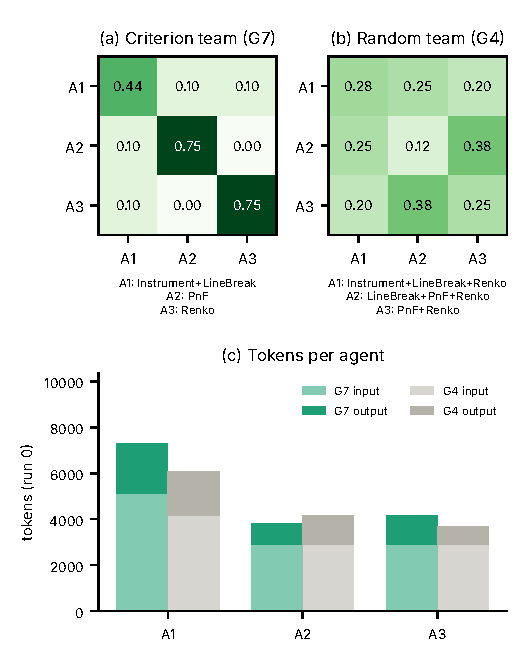
\includegraphics[width=\linewidth]{figures/teams.pdf}
\caption{Run 0 on stocktrends. (a, b) Cohesion (diagonal) and coupling (off-diagonal) between agents, as in MQ, for the criterion team and a random team of the same sizes; the classes each agent owns are listed below. (c) Input and output tokens per agent in that run.}\label{fig:teams}\end{figure}
